\begin{frame}
\begin{columns}
\column{0.3\textwidth}
\begin{pspicture}(-1.4,-1.4)(1.4,1.4)
\tiny
\pstVerb{100 dict begin /innerRad 1 def /outerRad 1.4 def}%
\fcStartIIIdScene
\fcSurfaceInScene[colorUV={0.8 0.9 1}, colorVU={0.7 0.7 1}, linewidth=0.4, iterationsU=17, iterationsV=1]{0 }{-1}{360}{1}{[u cos innerRad mul u sin innerRad mul v]}{}
\fcSurfaceInScene[colorUV={0.8 0.9 1}, colorVU={0.7 0.7 1}, iterationsU=17, iterationsV=1]{0 }{-1}{360}{1}{[u cos outerRad mul u sin outerRad mul v]}{}
\fcSurfaceInScene[colorUV={0.8 0.9 1}, colorVU={0.8 0.9 1}, iteraionsU=17, iterationsV=1]{0 }{innerRad}{ 360}{ outerRad }{[u cos v mul u sin v mul 1]}{}
\fcSurfaceInScene[colorUV={0.8 0.9 1}, colorVU={0.7 0.7 1}, iteraionsU=17, iterationsV=1]{0 }{innerRad}{ 360}{ outerRad }{[u cos v mul u sin v mul -1]}{}
\fcFinishIIIdScene[true]%
\only<2->{%
\fcLineIIId[linecolor=red, linewidth=2pt]{[0 0 1]}{[-720 17 div cos outerRad mul -720 17 div sin outerRad mul 1]}%
\fcPutIIId{[0 -0.3 0.9]}{$\alertNoH{2}{r_2}$}%
}%
\only<3->{%
\fcLineIIId[linecolor=red, linewidth=2pt]{[0 0 1]}{[0 cos innerRad mul 0 sin innerRad mul 1]}%
\fcPutIIId{[0.5 0 1.2]}{$\alertNoH{3}{r_1}$}%
}%
\only<4->{%
\fcLineIIId[linecolor=red, linewidth=2pt]{[360 17 div cos outerRad mul 360 17 div sin outerRad mul -1]}{[360 17 div cos outerRad mul 360 17 div sin outerRad mul 1]}%
\fcPutIIId{[360 17 div cos outerRad mul 360 17 div sin outerRad mul -1.2]}{$\alertNoH{4}{h}$}%
}%
\only<9->{% 
\fcLineIIId[linecolor=red, linewidth=2pt]{[-360 17 div cos outerRad mul -360 17 div sin outerRad mul 1]}{[-360 17 div cos innerRad mul -360 17 div sin innerRad mul 1]}%
\fcPutIIId{[1.4 -0.5 0.85]}{$\alertNoH{9}{\Delta r}$}%
}%
\only<10->{% 
\fcLineIIId[linecolor=red, linewidth=2pt]{[360 17 div 5.5 mul cos innerRad outerRad add 2 div mul 360 17 div 5.5 mul sin innerRad outerRad add 2 div mul 1]}{[0 0 1]}%
\fcPutIIId{[-0.5 1.4 1]}{$\alertNoH{10}{r}$}%
}
\pstVerb{end}%
\end{pspicture}
%the graphics here looks better:
%\ 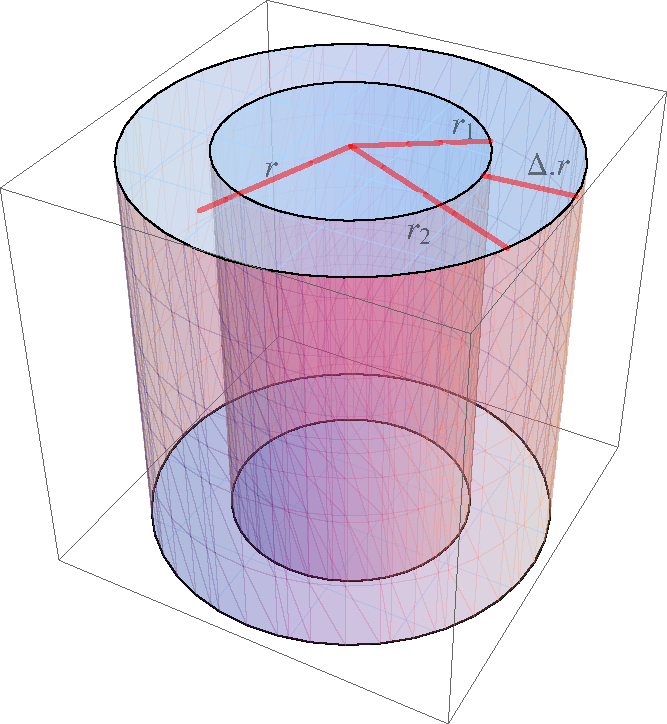
\includegraphics[height=4cm]{volumes/pictures/06-03-cylinder.pdf}%
%however I prefer to stay with internal graphics for the purposes of highlighting and uncovering things. 
%It should be possible to modify the internal 3d graphics to make it look as good as the original...
\column{0.7\textwidth}
\begin{itemize}
\item<1->  Consider a cylindrical shell with:
\item<2->  \alertNoH{2}{outer radius $r_2$},
\item<3->  \alertNoH{3}{inner radius $r_1$},
\item<4->  \alertNoH{4}{height $h$}.
\item<5->  $V_{\text{shell}} = \alertNoH{6}{V_{\text{outer cyl.}}} - \alertNoH{7}{V_{\text{inner cyl.}}} \uncover<6->{= \alertNoH{6}{ \pi \alertNoH{8}{r_2^2} h} - \alertNoH{7}{\pi \alertNoH{8}{r_1^2} h} } \uncover<8->{ = \alertNoH{11}{\pi} \alertNoH{8}{(\alertNoH{14}{r_2 - r_1})(\alertNoH{12}{r_2 + r_1})}\alertNoH{13}{h}}$.
\item<9->  Let $\alertNoH{9}{\Delta r = r_2 - r_1}$.
\item<10->  Let $\displaystyle r = \frac{r_2+r_1}{2}$.
\item<11->  Then $V_{\text{shell}} = \alertNoH{12}{2} \alertNoH{11}{ \pi} \alertNoH{12}{r}\alertNoH{13}{h}\alertNoH{14}{\Delta r}$.
\end{itemize}
\end{columns}
\end{frame}